\documentclass[conference]{IEEEtran}
\usepackage[USenglish]{babel}
\usepackage{graphicx}
\usepackage{cite}
\usepackage{amsmath}
\usepackage{graphicx}
\usepackage{graphics}
\usepackage{psfrag}
\usepackage{pstricks}
\usepackage{color}
\usepackage{amsmath}
\usepackage{rotating}
\usepackage{setspace}
\usepackage{cite} % ordena as citacoes
\usepackage[T1]{fontenc}
\usepackage{mathtools, cuted}
\usepackage{subfig}
\usepackage{caption}
%\usepackage{subfigure}
%\usepackage[export]{adjustbox}

%\ifCLASSINFOpdf
%\else
% * <jose.avalos@utec.edu.pe> 2017-07-01T20:45:07.865Z:
%
% ^.
%\fi
%\hyphenation{op-tical net-works semi-conduc-tor}

\newcommand{\x}{\mathbf x}
\newcommand{\q}{\mathbf q}
\newcommand{\f}{\mathbf f}
\newcommand{\e}{\mathbf e}


\begin{document}
%%%%%%%%%%%%%%%%%%%%% TITLE %%%%%%%%%%%%%%%%%%%%%%%%%%%%%%%%%%
%\title{Image-driven robot-based drawing system itation of Human Drawing by a NAO Robot}
\title{Autonomous Motion of a Mobile Robot based on Potential Fields and Polar Control}
\author{\IEEEauthorblockN{Jose-Maria Munoz, Emanuel S. Munoz, Oscar E. Ramos}
\IEEEauthorblockA{Department of Electrical Engineering, Universidad de Ingenieria y Tecnologia - UTEC, Lima, Peru}
}
% \author{\IEEEauthorblockN{Jose-Maria Munoz\IEEEauthorrefmark{1}, Jose Avalos\IEEEauthorrefmark{1}
% Oscar E. Ramos\IEEEauthorrefmark{1}}
% \IEEEauthorblockA{\IEEEauthorrefmark{1}Department of Electrical Engineering, Universidad de Ingenieria y Tecnologia - UTEC, Lima, Peru.}
% }
\maketitle
\begin{abstract}
  Autonomous motion of mobile robots is an open problem in robotics. One of the challenges consists in properly interpreting the information from the sensors, and another challenge is to adequately move according to this information.
%   The differential wheeled 
% robot is widely used for navigation tasks. However it has limitation in its
% motion because its non-holonomic constraints.
  In this work, we propose an algorithm which drives a mobile robot through a
  collision-free trajectory smoothly. The generation of trajectories is based
  on Artificial Potential Fields for the sensed environment, whose information
  is acquired using a depth sensor. The generated path is then followed using
  an iterative closed-loop feedback controller based on polar coordinates which
  % works for semi-trajectories so they can be guided from the vector forces of
  works guided by the vectors coming from the potential field. The robot can
  thus move autonomously to a desired position avoiding obstacles. Results were
  obtained using a dynamic simulator and also using Quanser's Qbot2 mobile
  robot.
  % from simulations in Gazebo software for the Kobuki model and
  % from the implementation of the algorithm in real Kobuki robot sensing with a
  % Lidar sensor.
\end{abstract}
\IEEEpeerreviewmaketitle
% \textbf{\textit{Keywords - NAO Robot, Inverse Kinematics, Image Processing, Drawing Imitation}}

\section{Introduction}

Autonomy in mobile robots is a current challenge in robotics since no flawless method for its implementation exists. All systems have to deal with the probability of the sensors and with the proper interpretation of the information. Mobile robots constitute an active field of research due to their applications such as exploration and navigation on the ground \cite{Bonin-Font2008}.
One particularly useful type of mobile robot is the differential wheeled robot since its dynamics and physical structure is not complex. However, their motion has to deal with their inherent non-holonomic constraints.
%application in navigation of these robots deals with some problems for the controllability of its kinematics.
%The robot is a non-holonomic system, so the controllability of these robots is difficult to achieve.
These constraints need to be taken into account when doing trajectory tracking in any environment. For example, the robot cannot achieve a goal smoothly because its orientation is significantly important to its motion. Some approaches to this solution has gone through different approaches \cite{Rubayat}. 
% In general, these approaches can be divided for the model in a different system of coordinates.
The usage of polar coordinates facilitates the control of the robot in a Cartesian coordinate system. Also, the control laws based on these coordinates have the potential to achieve an exponential stability smoothly through a closed-loop control \cite{Matoui}. However, the mathematical formulation of these control laws do not consider trajectory constraints. Moreover, polar control laws can be used for obstacle avoidance when used with appropriate frameworks. 
% if there are obstacles if it is stated middle goals in which the robot can avoid them. However, these middle goals must be formulated arbitrarily, which is not a good approach for the autonomy of the robot in a navigation task.

Practical applications of mobile robots deal with an environment, which by nature has different obstacles. Therefore, it is necessary to overcome this limitation of the control. There exist different approaches to solve the path planning problem. One of those approaches is the artificial potential field (APF) method \cite{Woods}. For non-holonomic robots, the path generated by this trajectory planner can be hard to follow through conventional control methods such as a classic PID controller. 
%or the two-wheeled robot, its non-holonomic problem impede a normal path planning through this method. The artificial attractive or repulsive forces formulate trajectories which the robot cannot follow through conventional control methods. 

In this work, we propose an autonomous motion framework based on potential fields and on polar control laws for the kinematics of a two-wheeled robot, so it can smoothly achieve a validated trajectory to reach a goal position. Experimental results of the proposed framework were obtained through the implementation of each individual controller in a Kobuki model using a dynamic simulator. The controllers were also used to implement autonomy on a real Kobuki robot powered with a Lidar sensor as shown in Fig.~\ref{fig:example-robot}.  The onboard controller of this robot was done using a Raspberri Pi3 computer.
% Posteriorly, the integration of the controllers for obtaining the proposed control is implemented in a real Kobuki robot powered with a Lidar sensor for obtainment of position obstacles. 
% This work is structured as follows. In section \ref{sec:robot_motion}, it is introduced the forward and inverse kinematics. Section  \ref{sec:APF} formulates the potential field equation for its application as well as it is stated the control laws in the polar coordinate system.Finally, the experimental results and conclusion are shown to give details of the implementation.

\begin{figure}%[h]
  \centering \footnotesize
  \subfloat
  {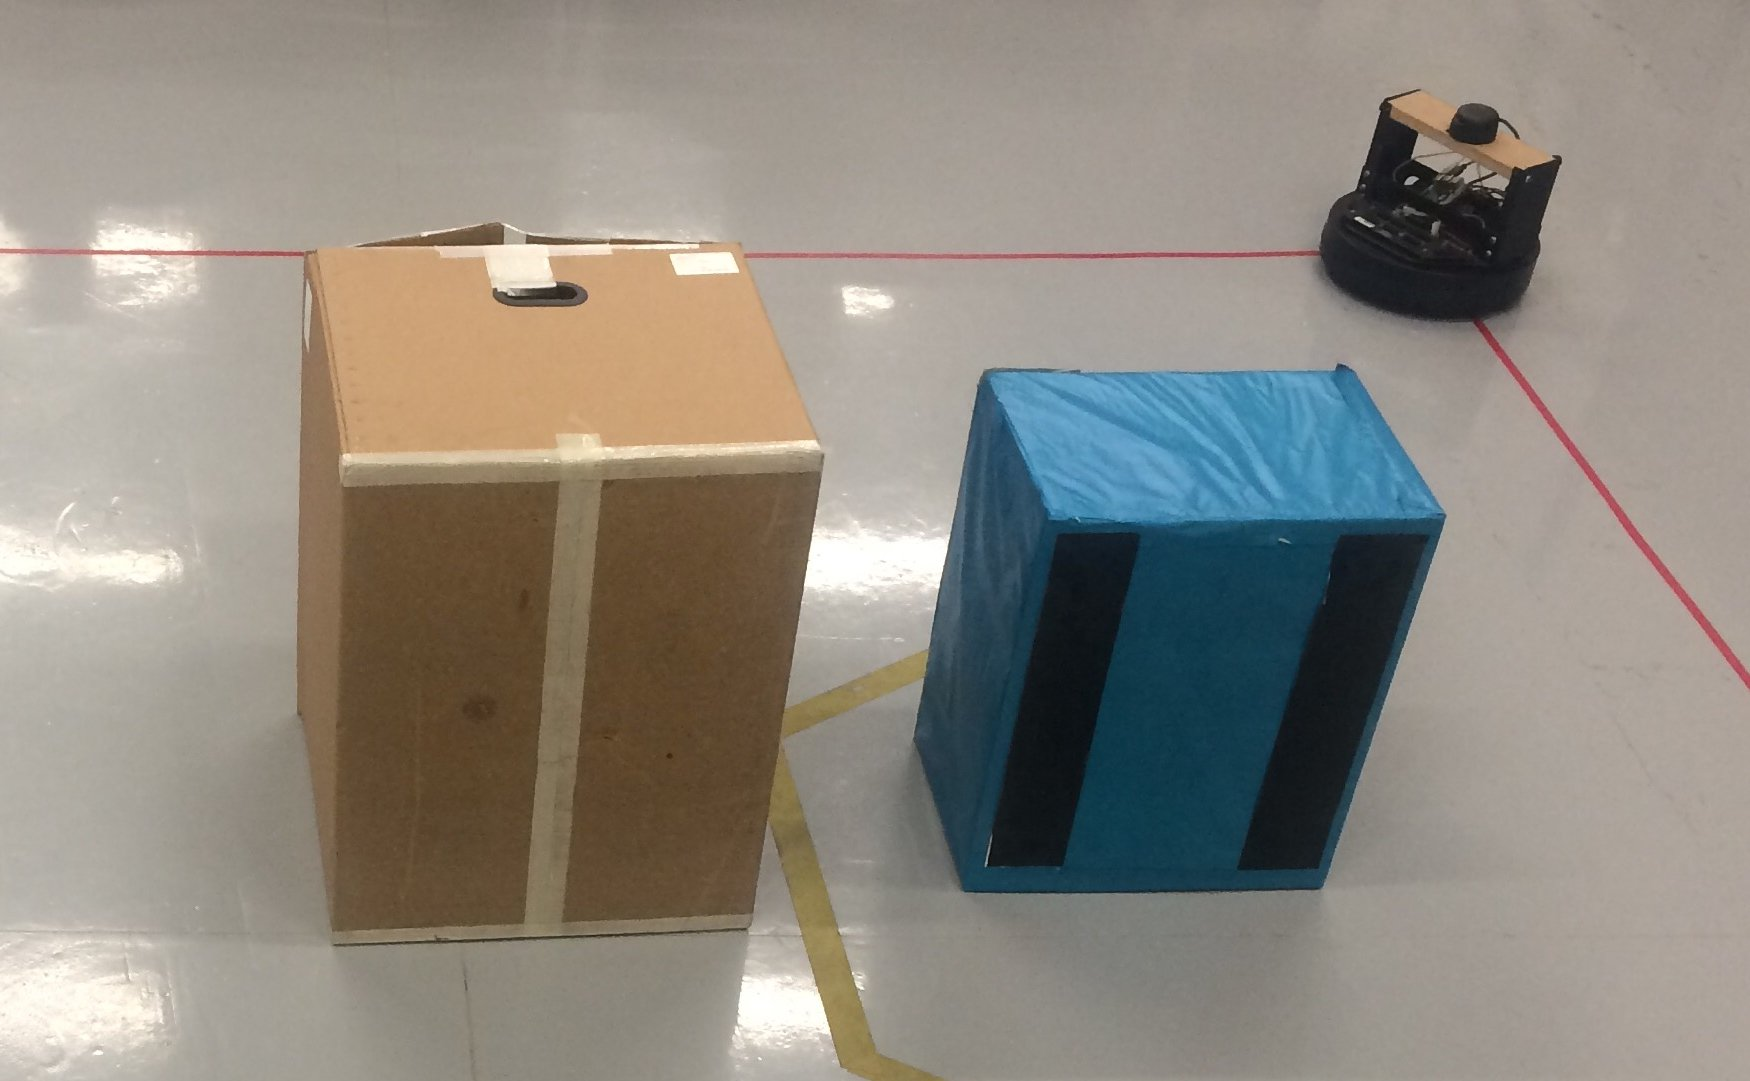
\includegraphics[width=0.3\textwidth]{kobuki}}
  \captionsetup{font=footnotesize}
  \caption{Front and top views of a generated motion for the model of a
    quadruped robot with a floating base: the robot rotates its body while
    lowering it, raising a frontal leg and maintaining the other three legs on
    the ground.}
  \label{fig:example-robot}
\end{figure}


\section{Robot Motion Generation}
\label{sec:robot_motion}

For navigation in a wheeled differential robot, it is necessary to control its motion appropriately. A classic way is using a PID controller in the Cartesian space. However, this control is usually ill-posed for a differential wheeled robot.
%In this section, the kinematics of the robot is recalled, and the control laws for its motion based on a polar approach is presented.
% In this section the control laws for its motion based on a polar approach is presented.
%\subsection{Polar controller}
An alternative way of achieving a softer control in position and orientation for a differential robot is using a linear control law for the feedback of the states based on polar coordinates. As Fig.~\ref{fig:Polar} shows, the polar coordinates associated with the robot are the following
\begin{align*}
  \rho &= \sqrt[]{(x_{d} - x)^2 + (y_{d} - y)^2}  \\
  \alpha &= \text{atan2}(y_{d} - y, x_{d} - x) - \theta  \\
  \beta &= -\text{atan2}(y_{d} - y, x_{d} - x) + \theta_{d}.
\end{align*}
where the variables are shown in~\ref{fig:Polar}. 
\begin{figure}%[h]
 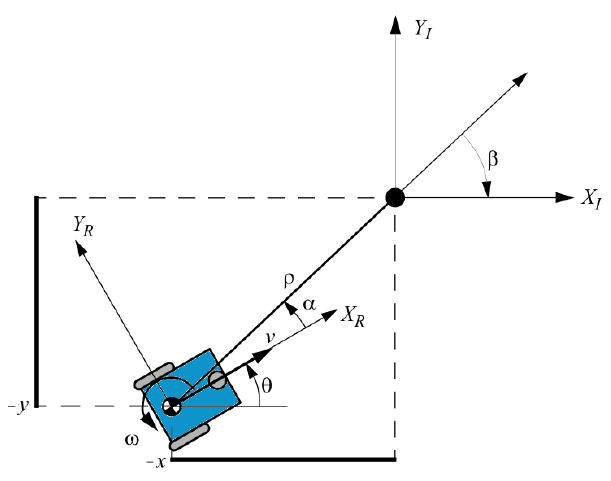
\includegraphics[width=0.5\linewidth]{control_polar.png}
 \centering\caption{Feedback control of states to a reference position}
 \label{fig:Polar}
\end{figure}
Considering the shown variables, the following control law can be used for the linear speed and for the angular velocity of the robot:
\begin{align*}
  v &= k_{\rho}\rho \\
  \omega &= k_{\alpha}\alpha + k_{\beta}\beta
\end{align*}
where $k_{\rho}$, $k_{\alpha}$, and $k_{\beta}$ are gain constants that need to be properly tuned.


\section{Path Generation}
\label{sec:APF}

To achieve autonomy, once the motion has been properly controlled, it is necessary to determine the path that it should track. This track in this case will be guided by an artificial potential scheme.

\subsection{Artificial Potential Field}
There exist several approaches in path planning through potential field. In this case, we opted for a one which considers some assumptions for its implementation. Given the potential field generates a force field, it is posteriorly used a guide to generate middle-goals for the polar control. In that way, it is only necessary the positions of the robot, the goal and the obstacles, so it could be generated a vector field from the sum of the attractive  and repulsive potential field.\\

\subsubsection{\textbf{Attractive Potential Field}}
The attractive potential field drives the robot to the goal position respect to the distance between them. Lets define a scalar potential field which depends on the distance between the current position of the robot $q$ and the goal position $q_{goal}$ as follows. 
\begin{equation}
	U_{att}(q) = \frac{1}{2} \zeta d^2(q,q_{goal})
	\label{eq:pot_attr}
\end{equation}

where  $\zeta$  is a parameter used to scale the effect of the attractive potential. The gradient of this field provides a vectorial field which points always to the desired goal position.

\begin{equation}
	\label{gradient_att}
	\begin{aligned}
		\nabla U_{att}(q) &= \nabla (\frac{1}{2}\zeta d^2 (q,q_{goal})),\\
		&=\frac{1}{2}\zeta \nabla d^2(q,q_{goal})\\
		&= \zeta(q - q_{goal})
	\end{aligned}
\end{equation}

The gradient vector points away from the goal with magnitude $\zeta$ at all points of the configuration space except the goal, where it is undefined. Starting from any point other than the goal, by following the negated gradient, a path is traced toward the goal. The equation \ref{gradient_att} is a vector based at $q$, points away from $q_{goal}$, and has a magnitude proportional to the distance from $q$ to $q_{goal}$.\\

\subsubsection{\textbf{Repulsive Potential Field}}

A repulsive potential keeps the robot away from an obstacle. The strength of the repulsive force depends upon the robot's proximity to the obstacle. The closer the robot is to an obstacle, the stronger the repulsive force should be. Therefore, the repulsive potential is usually defined in terms of distance to the closest obstacle $D(q)$.

\begin{equation}
	U_{rep}(q) = 
		\begin{cases}
			\frac{1}{2}\eta(\frac{1}{D(q)} - \frac{1}{Q*})^2, & D(q)\leq Q*, \\
			0, & D(q) > Q*,
		\end{cases}
	\label{eq:pot_rep}
\end{equation}

whose gradient is
\begin{equation}
	\nabla U_{rep}(q) = 
		\begin{cases}
			\eta (\frac{1}{Q*} - \frac{1}{D(q)})\frac{1}{D(q)^2} \nabla D(q), &D(q) \leq Q*,\\
			0 , &D(q) > Q*,
		\end{cases}
	\label{eq:force_rep}
\end{equation}

where the $Q* \in R $ factor allows the robot to ignore obstacles sufficiently far away from it and the $\eta$ can be viewed as a gain on the repulsive gradient. These scalars are usually determined by trial and error.


\section{Results}
The proposed methodology was tested on a real Kobuki mobile robot. ROS was used to program the mobile robot. This section is divided into two subsections which are:

\subsection{Artificial Potential Field}

Potential field was implemented so that you can perform different tasks in different situations and thus have a robust behavior. This algorithm works with forces of atrraccion and repulsion. The first is used to reach the desired position and the second force is to avoid obstacles. These forces were decomposed in magnitude and direction so that the robot can take semi desired positions for each iteration.
To check the efficiency of the algorithm, it was simulated graphically in a workspace where the vector field was projected, indicating the potential field algorithm forces for different positions of the obstacles and the desired position.The forces of atrraccion can be observed in Figure \ref{f:apf}(a), where the desired position is $ (10,4) $ and the initial position of the robot is $ (2,18) $. The white points within the image refer to the desired semi-positions forming the path of the robot. You can also see that all the arrows in the vector field are in the direction of the robot's goal. Likewise, also in Figure \ref{f:apf}(b) you can see three obstacles that are distributed in different positions of the workspace. Each obstacle is projected as a red circle due to its high magnitude within its potential field, where the forces point outward in each obstacle. Finally, for the force of navigation, the forces of attraction and repulsion had to be superimposed, as shown in Figure \ref{f:apf}(c). Where the white points is the trajectory that the robot would generate assuming that this robot has a controller that overcomes non-holonomicity without having restrictions for its movement.

%Potential field fue implementado para que pueda realizar diferentes tareas en diversas situaciones y así tener un comportamiento robusto. Este algoritmo trabaja con fuerzas de atrraccion y repulsion. El primero es utilizado para llegar a la posicion deseada y la segunda fuerza es para evitar obstaculos. Estas fuerzas fueron descompuestas en magnitud y direccion para que el robot pueda tomar semi posiciones deseadas para cada iteracion.
%Para comprobar la eficiencia del algoritmo se simulo de forma gráfica en un espacio de trabajo donde se proyectó el campo vectorial indicando las fuerzas del algoritmo potential field para diferentes posiciones de los obstaculos y de la posicion deseada. 
%Las fuerzas de atrraccion se pueden observar en la Figura \ref{f:apf}(a), donde la posición deseada es $(10,4)$ y la posicion inicial del robot es $(2,18)$. Los puntos de color blanco dentro de la imagen hacen referencia a las semi posiciones deseadas formando la trayectoria del robot. Tambien se puede ver que todas las flechas,del campo vectorial,estan en direccion hacia la meta del robot. Asimismo, también en la Figura \ref{f:apf}(b) se puede observar a tres obstaculos que estan distribuidos en diferentes posiciones del espacio de trabajo. Cada obstaculo se proyecta como un circulo rojo debido a su alta magnitud dentro de su campo potencial, donde las fuerzas apuntan hacia afuera en cada obstaculo. Finalmente, para la fuerza de navegacion se tuvo que superponer las fuerzas de atraccion y repulsion como se observa en la Figura \ref{f:apf}(c). Donde los puntos blancos es la trayectoria que generaría el robot asumiendo que este robot tiene un controlador que supera la no holonomicidad no teniendo restricciones para su movimiento.

\begin{figure}[ht!]
  \centering
  \subfloat[Attractive Force]{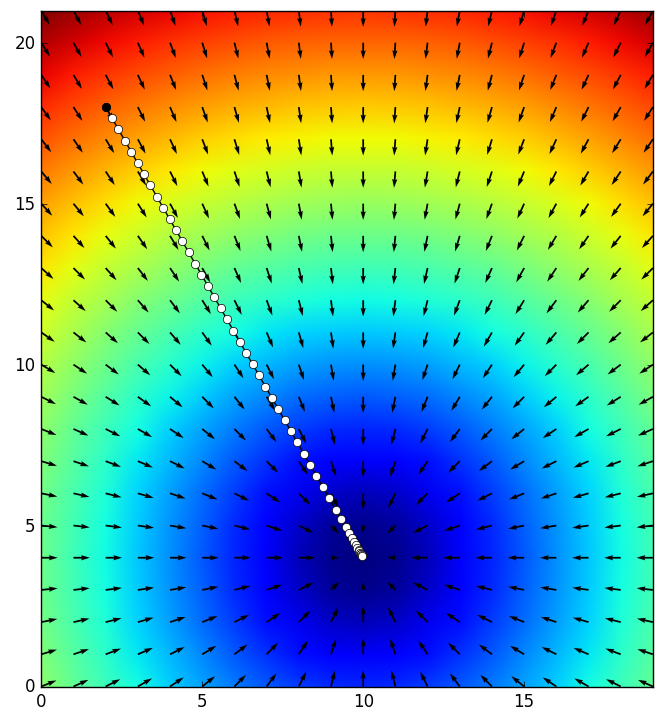
\includegraphics[width=40mm]{attr_force2.png}}
  ~\subfloat[Repulsive Force]{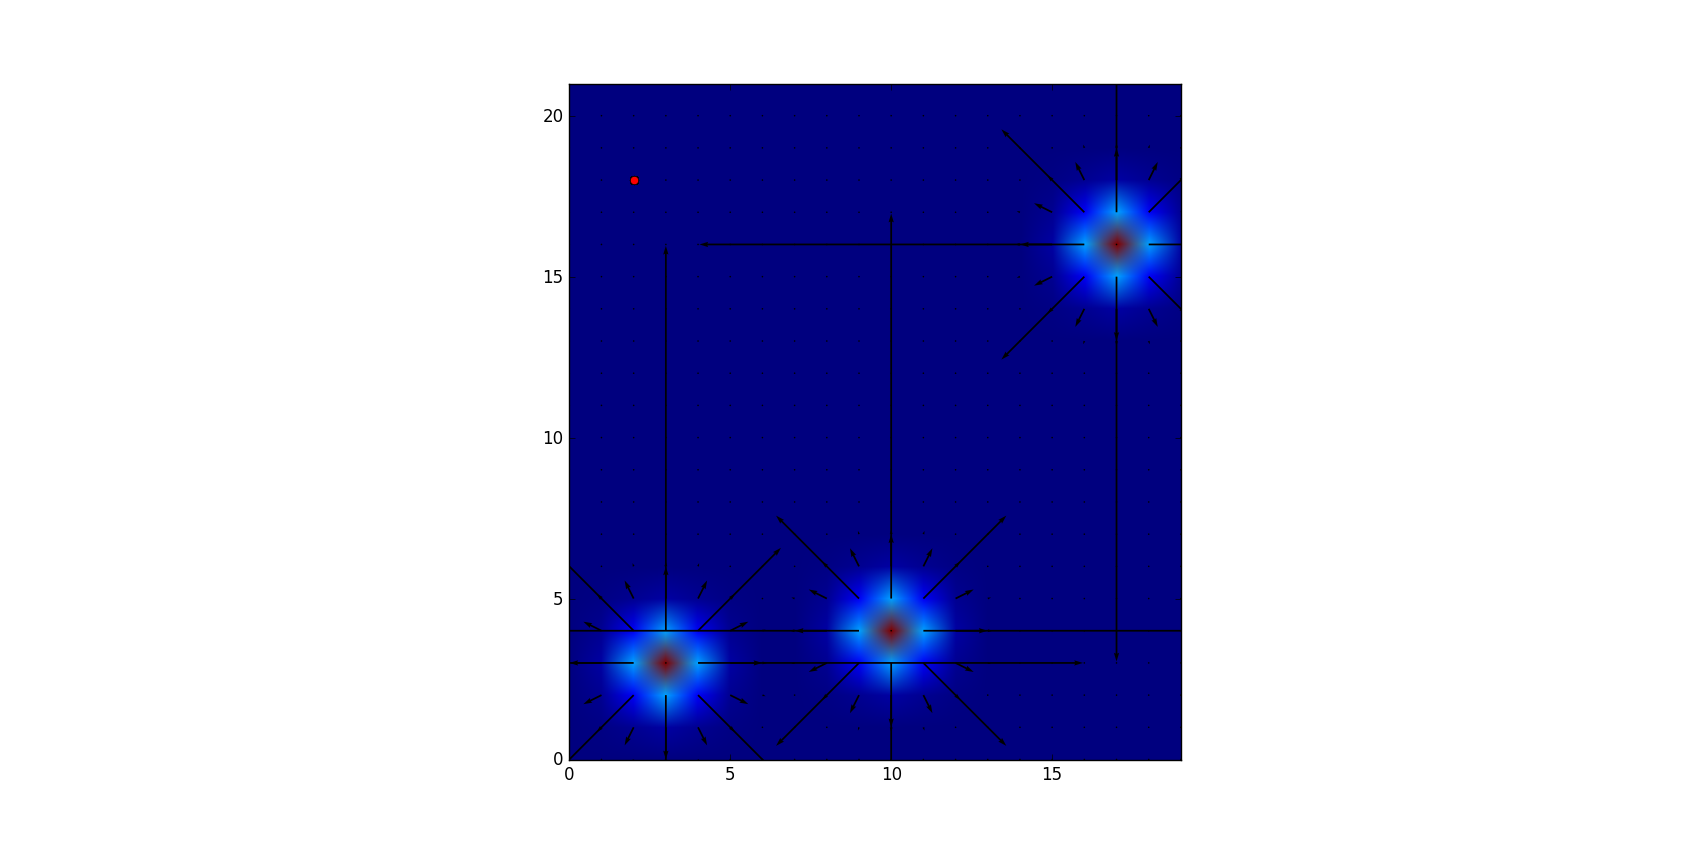
\includegraphics[width=40mm]{rep_force.png}}\\
  \subfloat[Navigation Force]{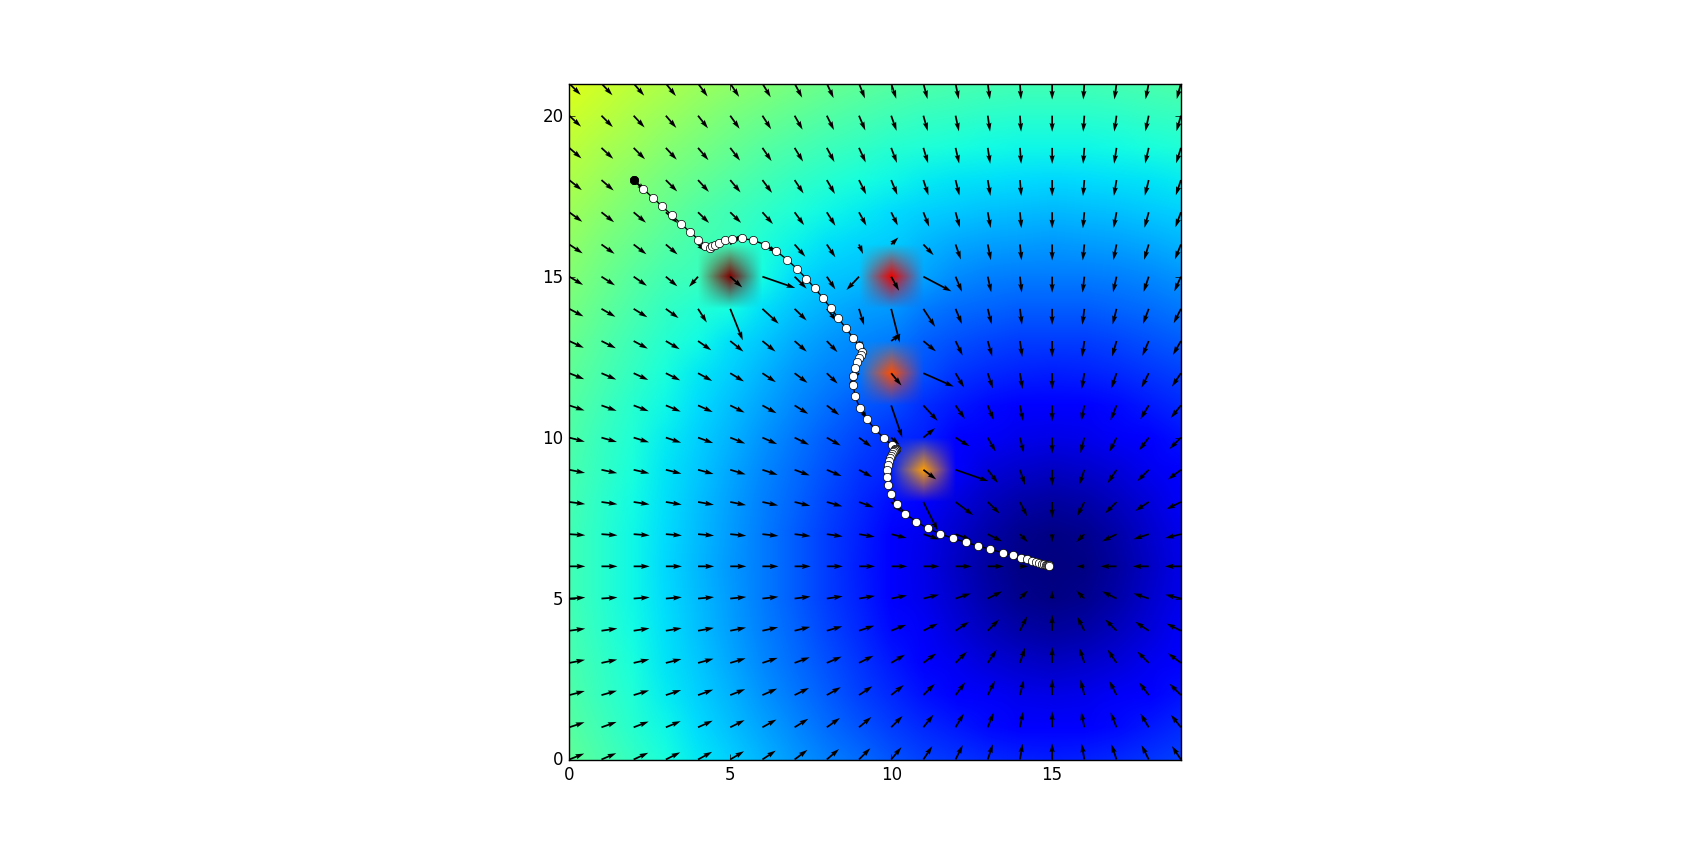
\includegraphics[width=40mm]{nav_force.png}}
%\subfloat[Attractive Force]{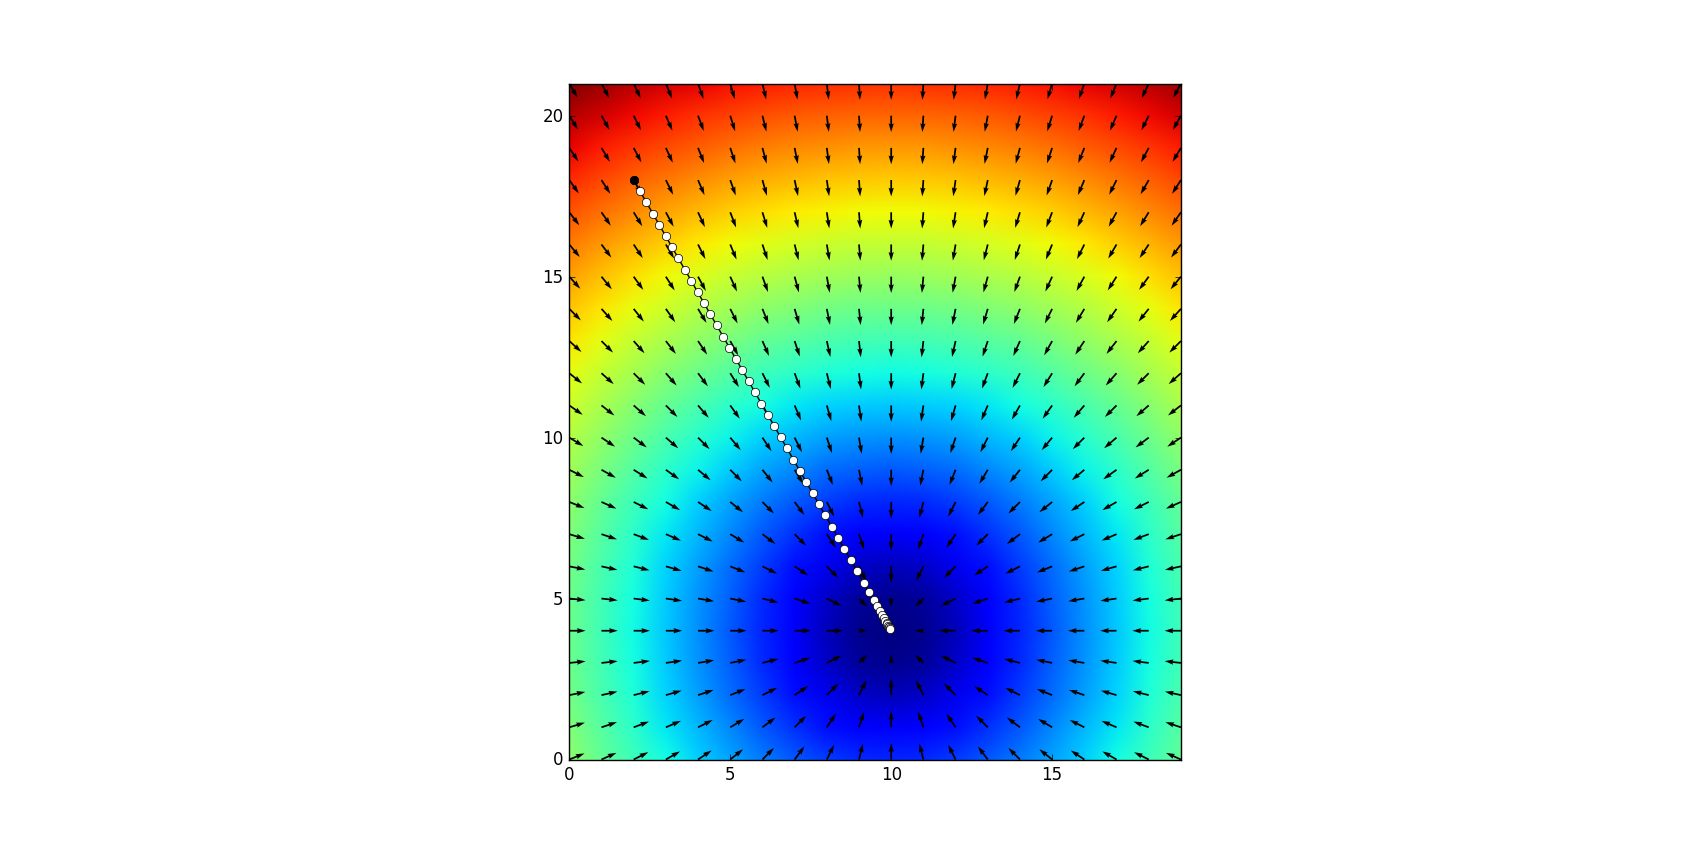
\includegraphics[width = 150mm]{attr_force.png}}
  \caption{Potential Field Algorithm} \label{f:apf}
\end{figure}

\subsection{Polar controller}

The polar controller was implemented for the Kobuki motion in a virtual workspace in Gazebo with no obstacles. The prompt of the proofs was the robot to achieve a given a random goal position.  It was considered a start position in the origin of the frame and the desired position ($x,y,\theta$) respect to the same inertial frame. The state variables (velocity, position and orientation) of the robot was obtained from odometry. The performance of the robot for one of the experimental cases is shown in the following figures.

The graphical results show the performance of the robot for a goal position ($x = 3,y = 3$) and orientation ($\theta = 90°$). The start time of simulation is approximately 7 seconds because of a delay of the software. For every figure, the variation of the variable is immediate and in a homogeneous convergence time. In contrast, the Figure \ref{f:polar}(a) shows a rapid convergence of the position compared to the other variables. In the same way, in Figure \ref{f:polar}(c), there is a peak in the curve which diverges from the goal orientation. These results proves an over-dependence of the controller to the position instead of the orientation. This characteristic is mainly upward for a navigation resolution.

\begin{figure}
	\centering
	\subfloat[time vs position]{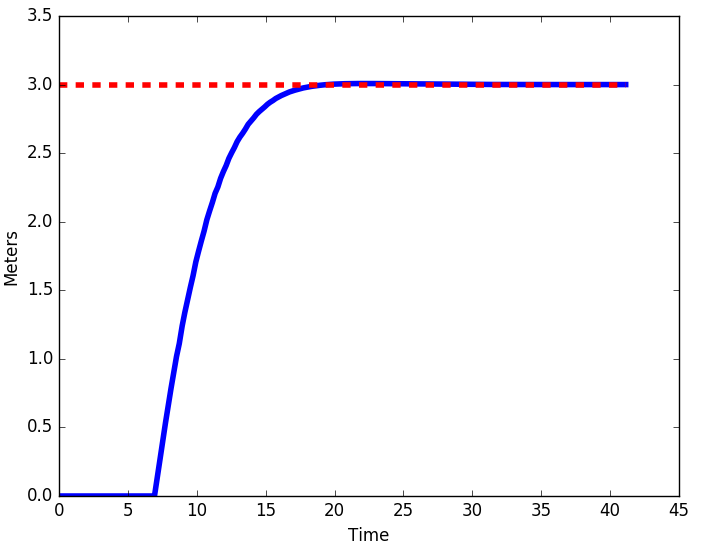
\includegraphics[width = 40mm]{tvsxy_tesis.png}}
	~\subfloat[time vs linear velocity]{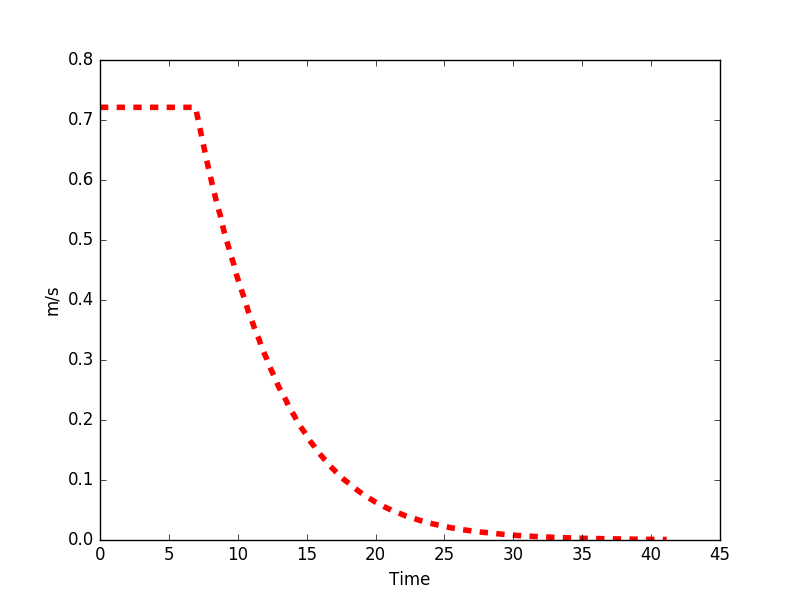
\includegraphics[width = 40mm]{tvsv_tesis.png}}\\
	\subfloat[time vs theta]{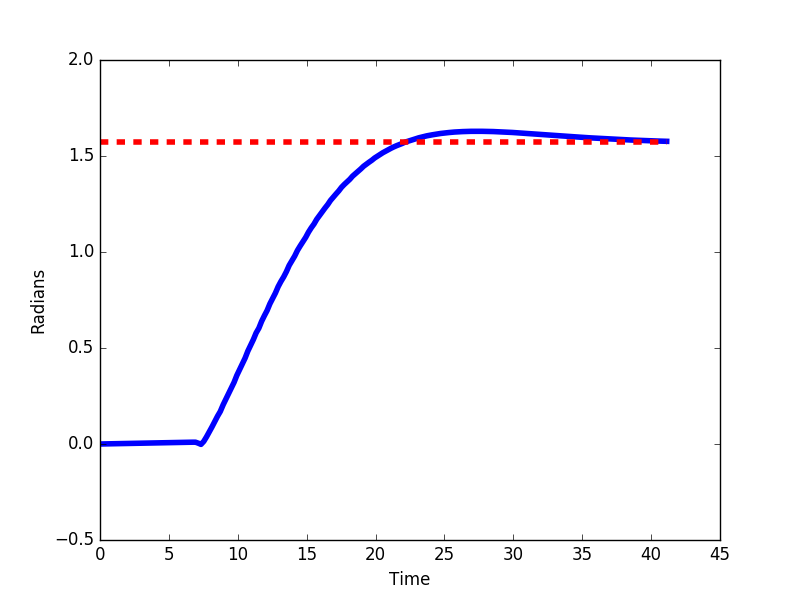
\includegraphics[width = 40mm]{tvstheta_tesis.png}}
	~\subfloat[time vs angular velocity]{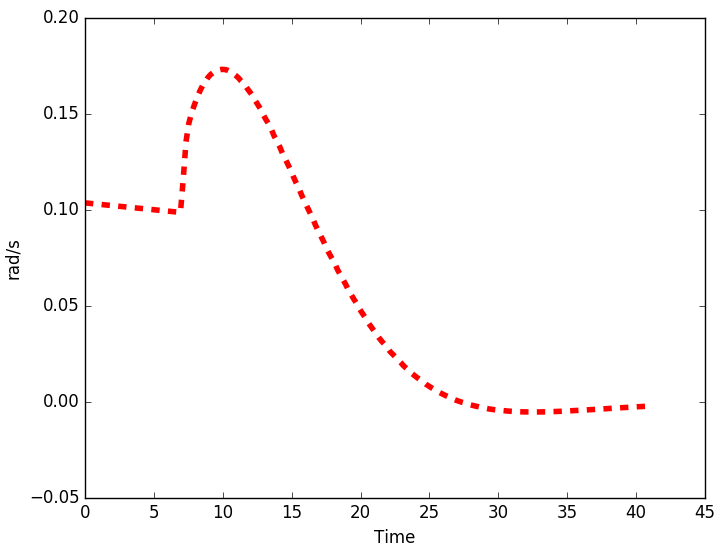
\includegraphics[width = 40mm]{tvsomega_tesis.png}}
	\caption{Polar controller for desired position $x=3, y=3, \theta=90°$} \label{f:polar}
\end{figure}

\subsection{Autonomous Navigation}
The proposed controller was implemented through an iterative algorithm for the Kobuki robot in a fixed environment. The algorithm takes middle goal position iteratively through the artificial potential field and it is drived by the polar controller to achieve them. We exposed to the robot to different obstacles whose positions were stated from a measurement of the physical of the environment, so it was not sensed by the robot. The performance of the robot is  shown in the following figures:

Figure \ref{f:kbki}(a) is composed of the attractive forces for every position(red dots) in which the algorithm is iterated in the two-dimensional environment within robot motion. It proves that for every position the attractive potential field drives the robot to the goal position. The trajectory shown in this figure is not forward to the goal because of the obstacles, which are not considered for the attractive APF. 

Figure \ref{f:kbki}(b) is composed for the repulsive forces for every iteration in the same 2D environment. The obstacles are shown in the graphic as green markers. The forces are only applied, as it was formulated above, for less than a arbitrarily range (for this result it was considered 1 meter). For each obstacle, the magnitude of the forces  increases as long as the robot is closer to it. Also, its direction points toward to the position of the robot, so it bring an opposite force to the attractive potential field.

Figure \ref{f:kbki}(c) shows the superposition of the forces with the actual obstacles. Each forces provides a middle goal position for the robot, thus it is the input variable for the polar controller. Even though the forces close to the obstacles have a high rate of change, the trajectory is smooth. It demonstrates the effectiveness of the polar controller despite its non-holonomic charateristic. 
\begin{figure}
	\centering
	\subfloat[Attractive force applied to the mobile robot]{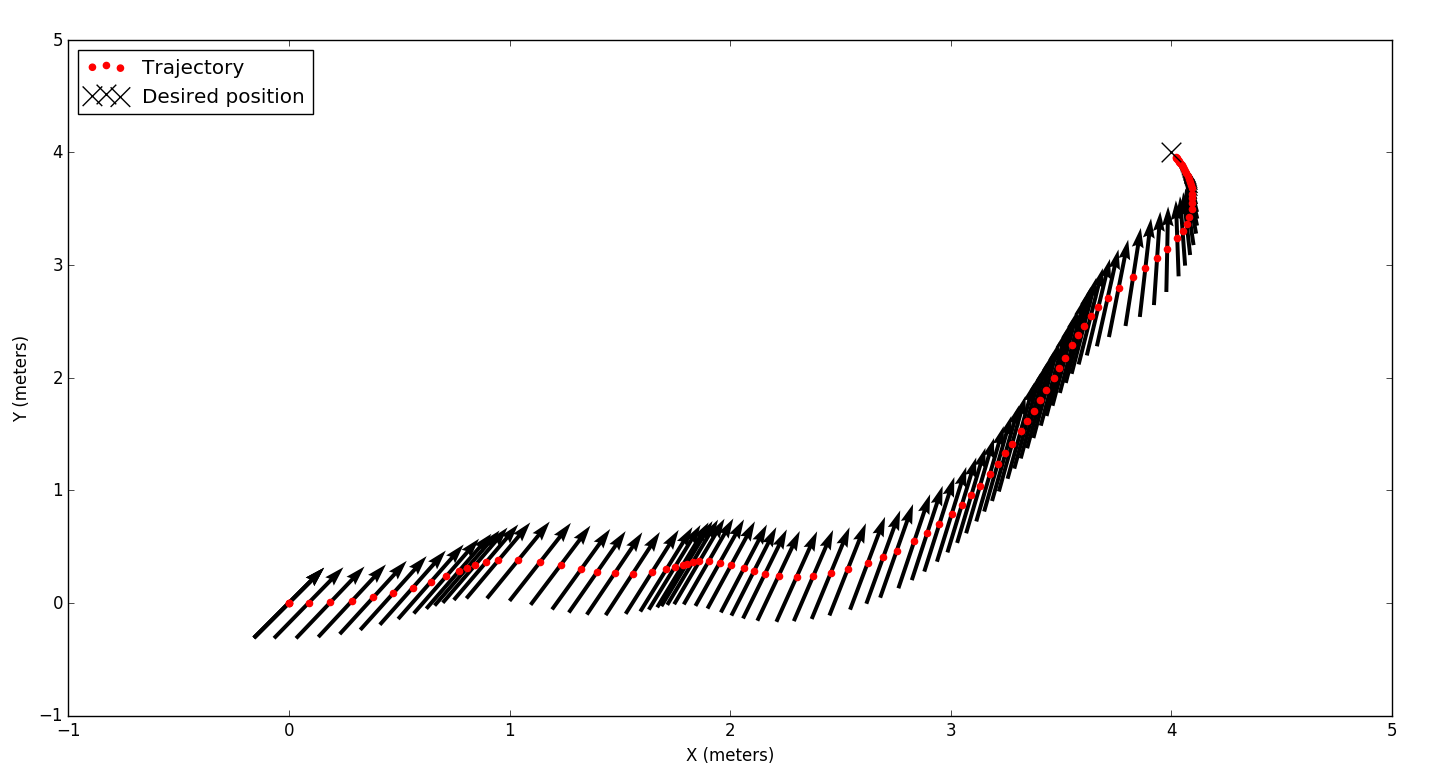
\includegraphics[width = 70mm]{attr_kbki.png}}\\
	\subfloat[Repulsive force applied to the mobile robot] {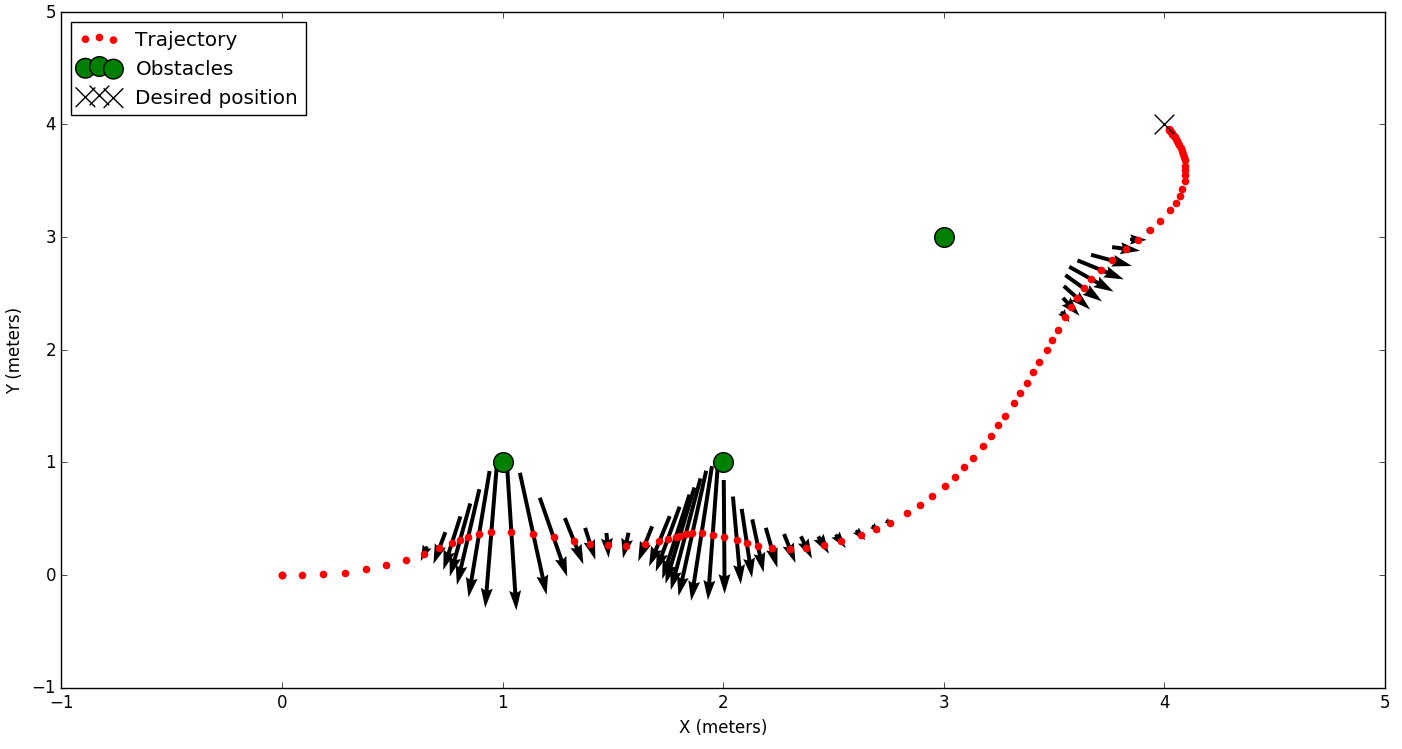
\includegraphics[width = 70mm]{rep_kbki.png}}\\
	\subfloat[Navigation force applied to the mobile robot]{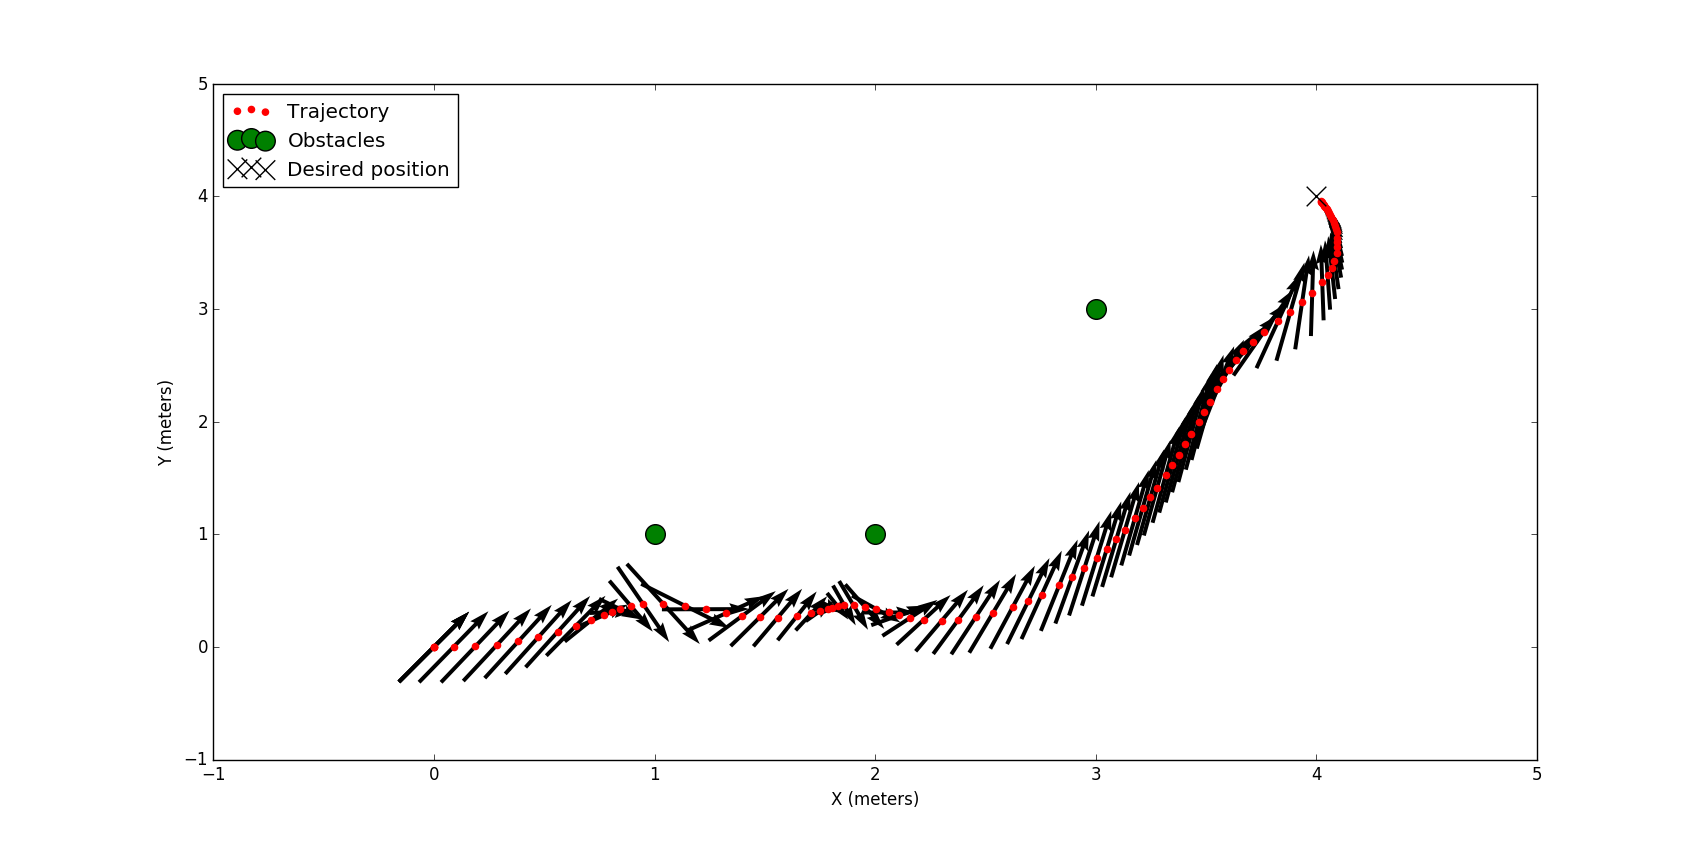
\includegraphics[width = 70mm]{nav_kbki.png}}
	\caption{Autonomous navigation implemented on Kobuki} \label{f:kbki}
\end{figure}

\subsection{Autonomous Navigation with Lidar}
For this section we worked with a lidar (RPLidar A2), which was installed on top of the kobuki. The proposal was to use the lidar to detect obstacles every time it moves.
Using ROS, he subscribed to the topic called / scan to obtain the measuring ranges of the sensor. With these values, a conversion of polar coordinates to Cartesian coordinates was made, in order to know the positions of the obstacles within the workspace. Then it was necessary to create a message in ROS and also a topic to be able to publish the Cartesian coordinates obtained from the 2D map generated by the lidar.
In order for the kobuki to be able to move on the map generated by the lidar sensor, the reference system of the robot must be taken to the reference system of the lidar. Once this is done, the autonomous navigation algorithm is subscribed to the coordinates sent by the lidar and thus can generate its own trajectory avoiding obstacles.
To perform this test, two boxes were placed in the workspace. The position was placed as goal ($ x = 4, y = 0 $).In Figure \ref{f:kbki_lidar}(a) you can see the path of the robot in blue and the arrows that indicate the force of the robot that bring the robot to the desired position. Also, in Figure \ref{f:kbki_lidar}(b) you can see the green dots that represent the environment where the kobuki is moving and you can also see the arrows that go out avoiding the kobuki can hit the boxes. Finally in Figure \ref{f:kbki_lidar}(c) you can see the navigation force that makes the robot can move autonomously.
\begin{figure}
	\centering
	%\subfloat [Kobuki with lidar in workspace]{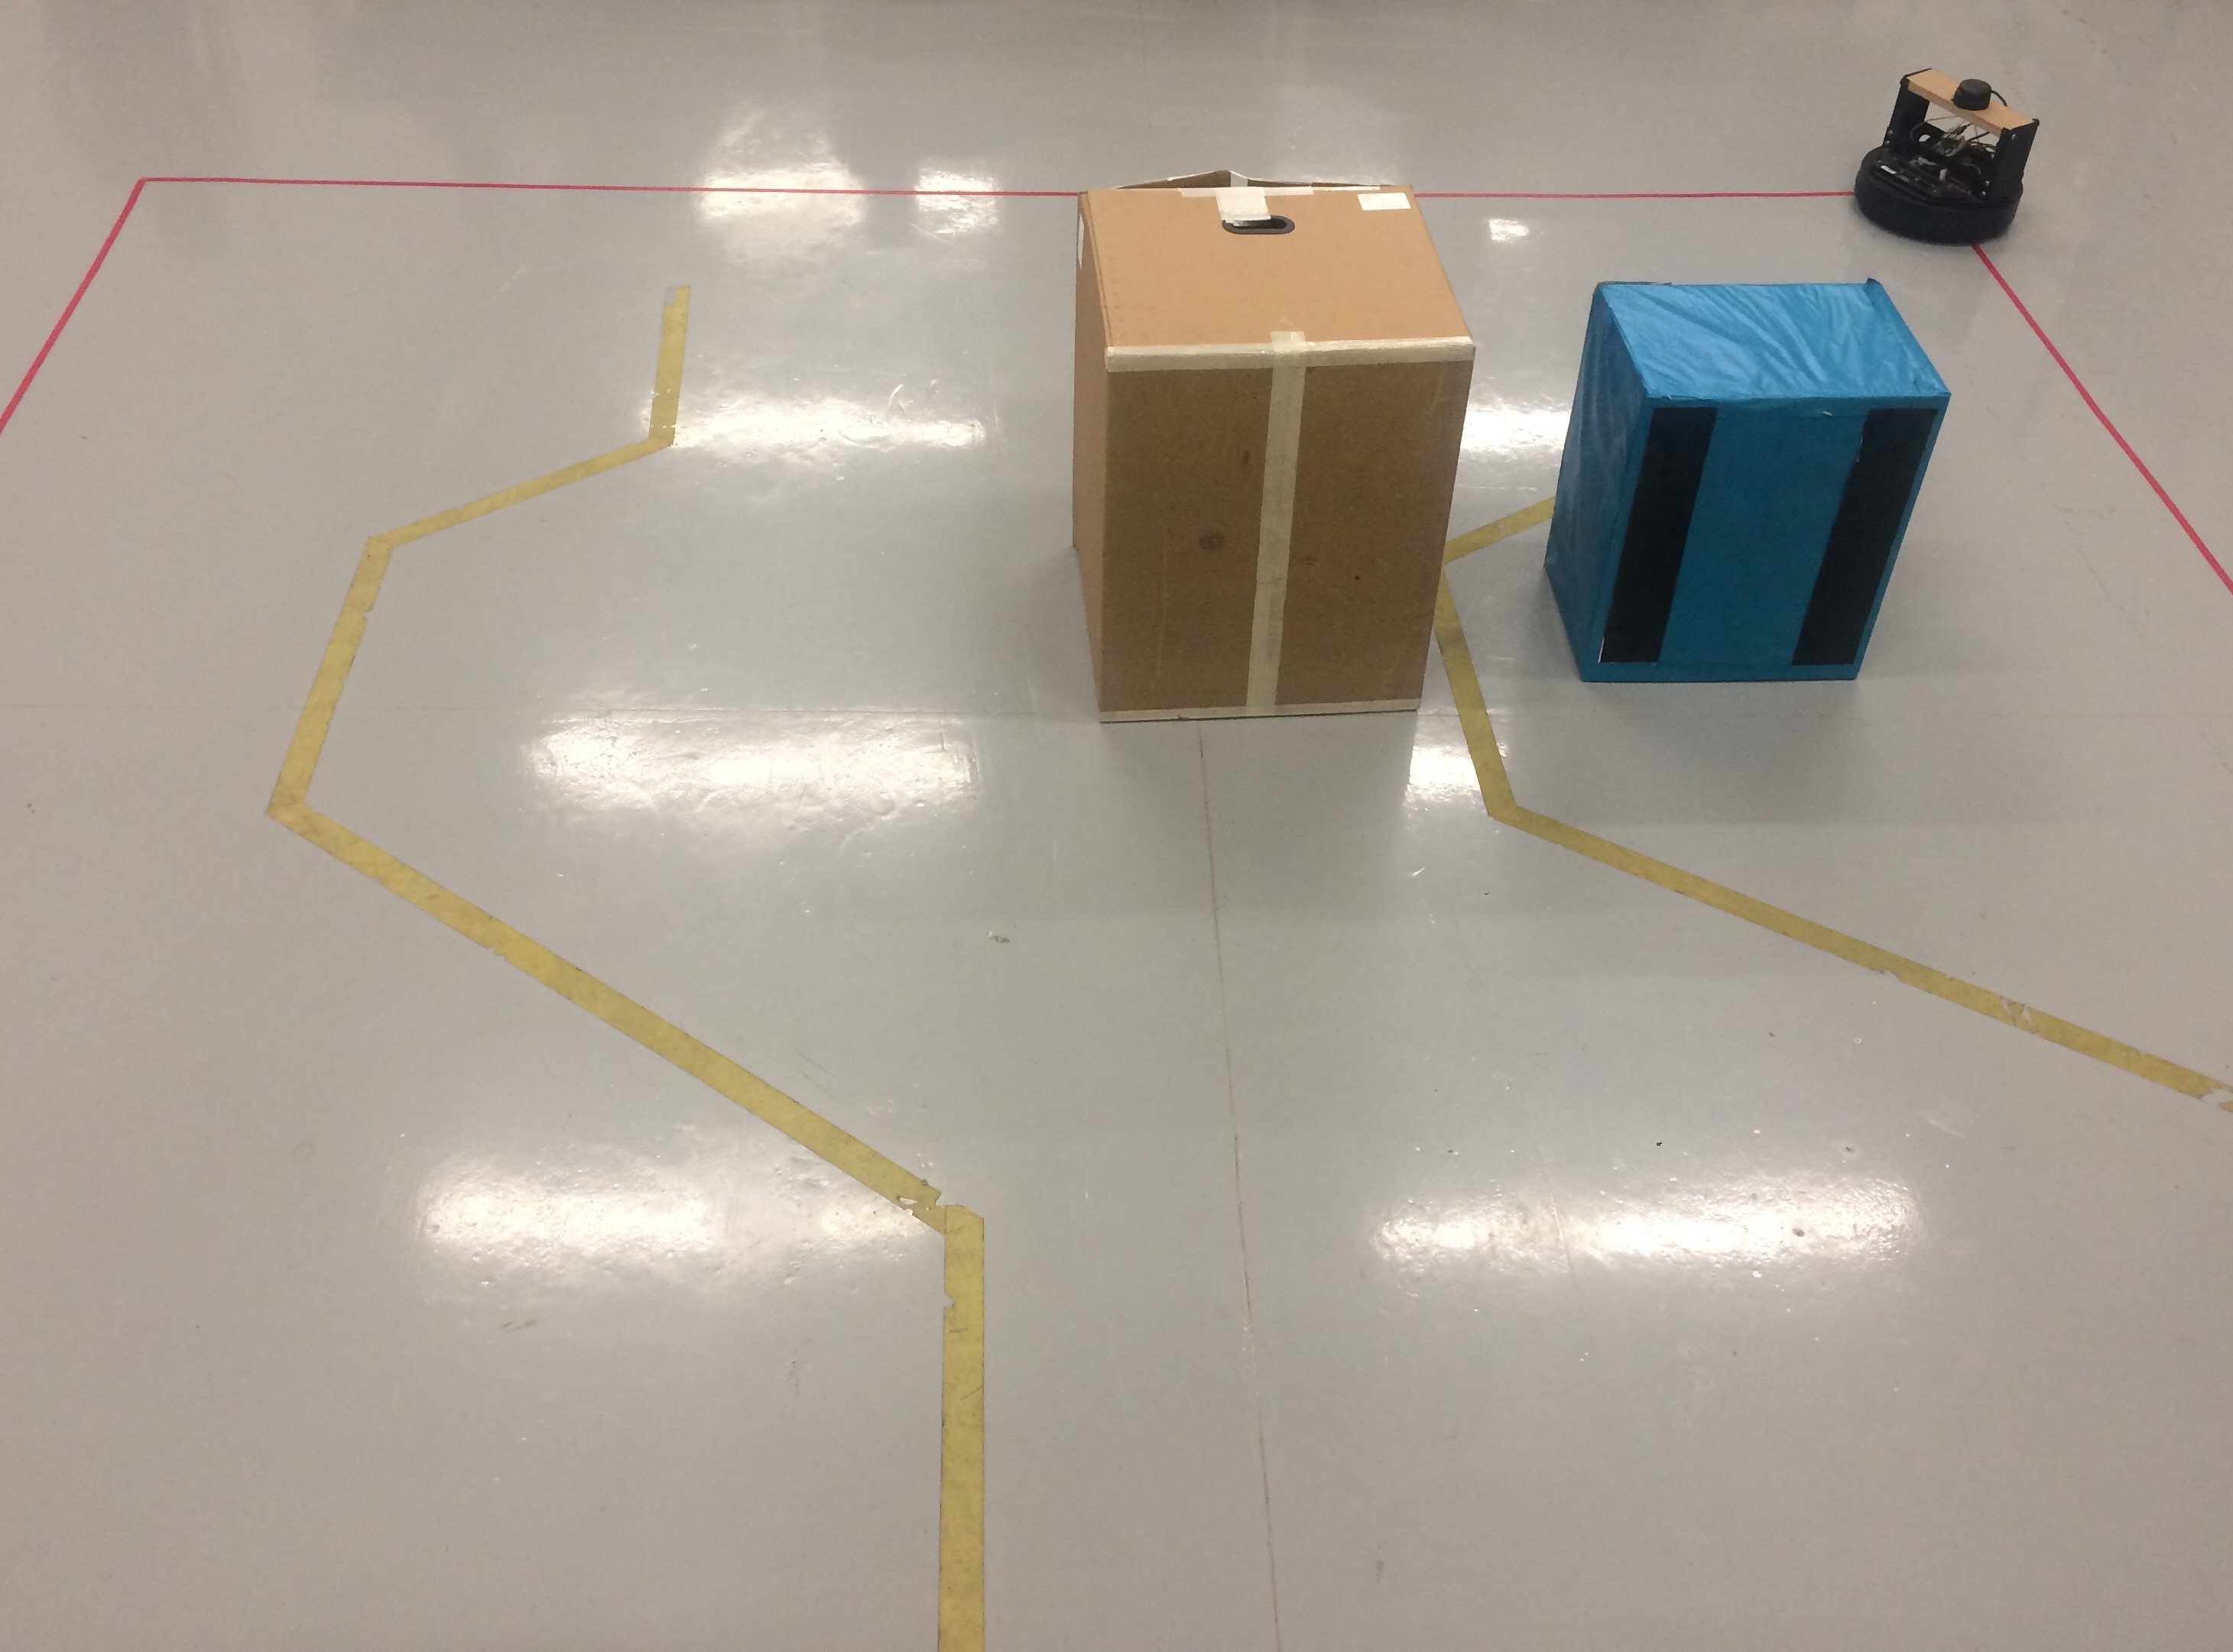
\includegraphics[width = 70mm]{kobuki_201.jpg}}\\
	\subfloat[Attractive force applied kobuki with lidar]{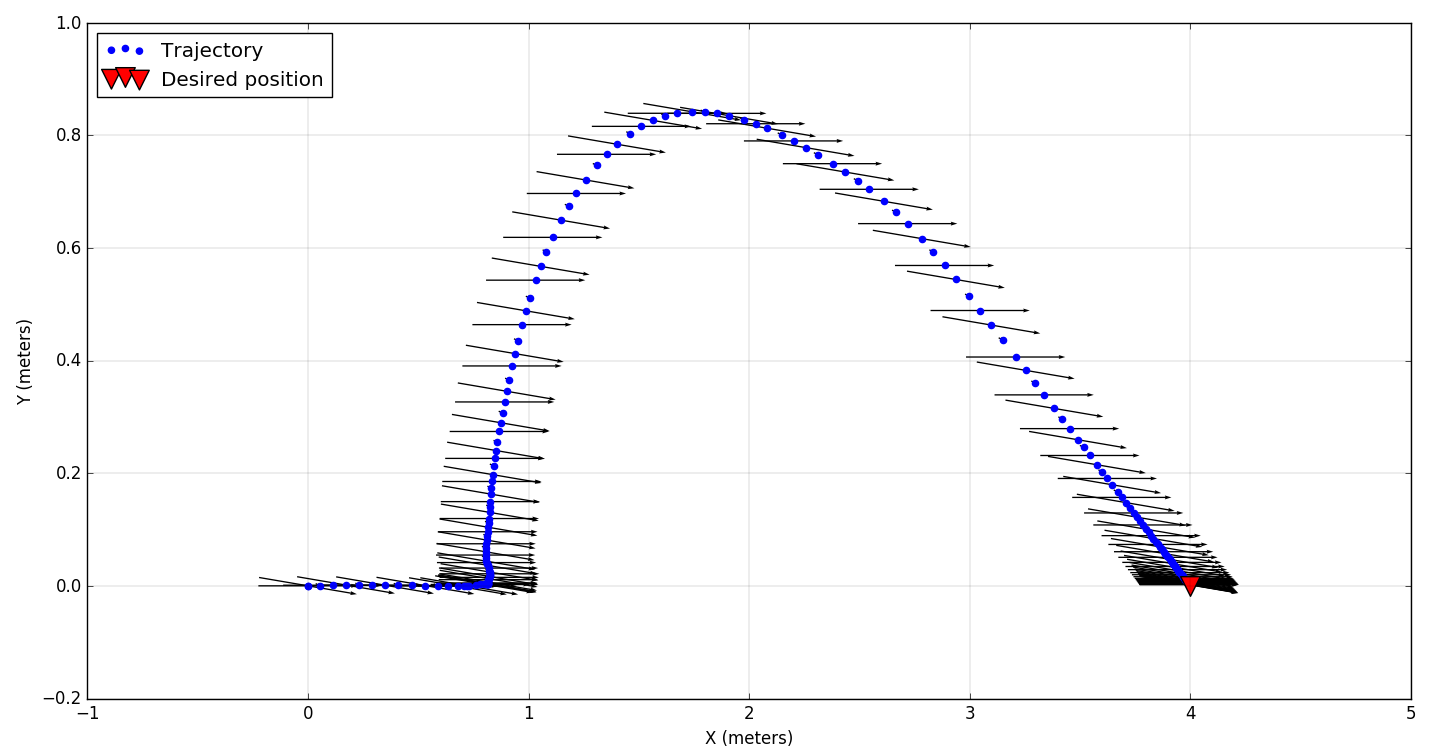
\includegraphics[width = 90mm]{fattr_lidar.png}}\\
	\subfloat[Attractive force applied kobuki with lidar]{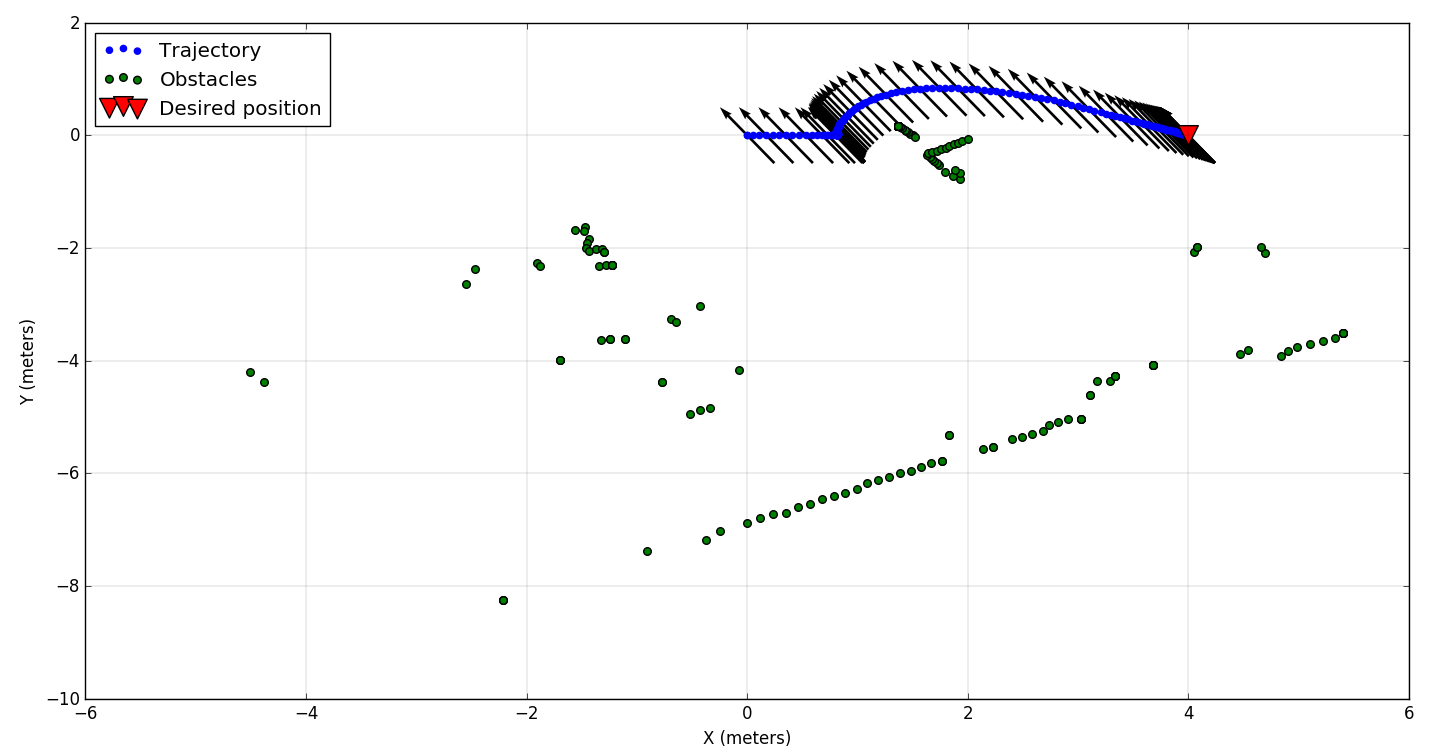
\includegraphics[width = 90mm]{frep_lidar.png}}\\
	\subfloat[Attractive force applied kobuki with lidar]{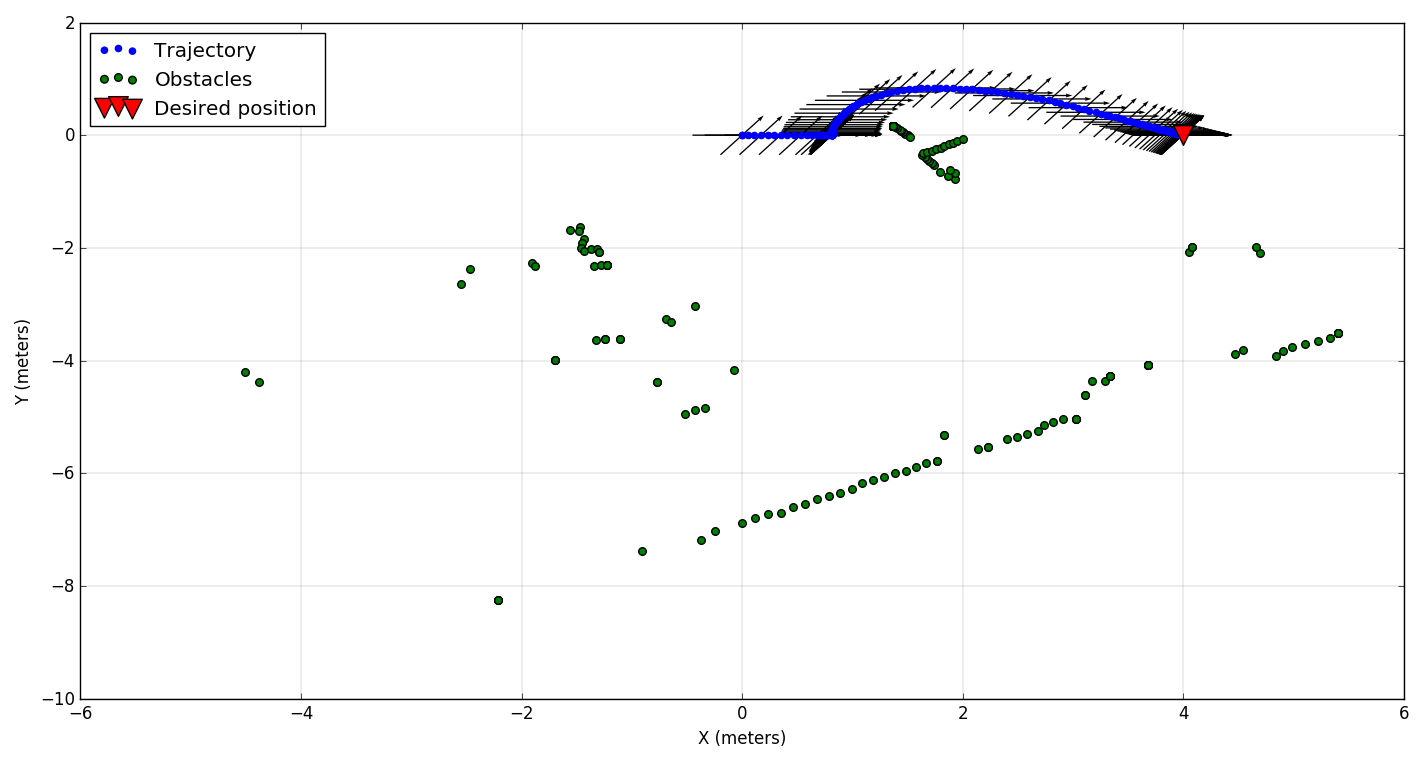
\includegraphics[width = 90mm]{fnav_lidar.png}}\\
	\caption{Autonomous navigation with lidar implemented on Kobuki} \label{f:kbki_lidar}
\end{figure}

\section{Conclusion}
\label{sec:conclusion}
We presented a controller based on Artificial Potential Field and a closed-loop feedback controller for navigation tasks of a differential drive robot. The motion controller differs from other works because it bases its frame in polar coordinates. Results for the motion controller proved to be a solution to the non-holonomic constraints that the robot presents. In the same way, the performance of the robot in simulation shows its rapid convergence through smooth trajectories.
Tests on the Kobuki robot show successful results. It also demonstrates the robot's autonomy despite the unknown configuration of the environment, since only odometry is used. It is demonstrated that by placing the lidar on the Kobuki robot, it can decide its obstacles in real time and can evade them without any problem reaching the goal.
\bibliographystyle{IEEEtran}
\bibliography{biblio.bib}
\end{document}

% Prueba
